\section{Frequency summation and the simultaneous Gaussian trace}
\label{e:section}

Put $s=n/(2(n+1))$.  We first turn \Cref{w:weak} into a
short-time estimate for exact extensions.  We then sum the frequencies on a
single dyadic time tree.  This order matters: maximizing separately at each
frequency would give a stronger frequency norm than $H^s$.
Throughout this section
\[
 S(t)f(x)=(2\pi)^{-n}\int_{\R^n}
       e^{ix\cdot\xi-it|\xi|^2}\widehat f(\xi)\dd\xi
\]
when $\widehat f$ has bounded support.  For general $f\in L^2$, $S(t)f$
initially denotes its $L^2$ equivalence class.

\subsection{Exact data and compact arrays}

\begin{lemma}[Compact layers for bounded-frequency data]
\label{e:compact-layers}
Let $g\in L^2(\R^n)$ have support in a fixed bounded frequency box, and let
$L\ge1$.  On $|T|\le C L^2$, its extension is a sum of compact arrays of
scale $L$,
\[
 \mathcal E g(X,T)=\sum_{q\in\Z^n} U_q(X,T).
\]
For any prescribed finite profile derivative order $J$ and any $A>0$, the
arrays can be chosen with uniformly bounded $C^J$ native profiles and
coefficient energies
\begin{equation}
 E_q\le C_{A,J}\braket{q}^{-2A}\norm{g}_2^2.
 \label{e:layer-energy}
\end{equation}
Each fixed $q$ has uniformly bounded phase-space multiplicity.  Finite
coefficient truncations converge uniformly on the stipulated time range,
and the sum in $q$ also converges uniformly.  Consequently any homogeneous
weak $L^p$ estimate for these compact arrays passes to $\mathcal E g$
without a power of $L$ or a count of layers.
\end{lemma}

\begin{proof}
Here $\mathcal E g$ uses the same Fourier normalization as $S(t)$; fixed
normalizing constants below are harmless.  Choose a smooth partition
$\sum_\theta\chi_\theta=1$ on the frequency box, with bounded overlap and
caps of side $L^{-1}$ centered at $\omega_\theta$.  In a fixed larger box
$B\subset\R^n$ form
\[
 G_\theta(\zeta)=L^{-n/2}
        (\chi_\theta g)(\omega_\theta+\zeta/L),
\]
extended by zero.  Its Fourier-series coefficients $c_{\theta,m}$ satisfy
\begin{equation}
 \sum_{\theta,m}|c_{\theta,m}|^2\le C\norm{g}_2^2
 \label{e:parseval}
\end{equation}
by Parseval and bounded overlap.  If $\psi_\theta$ is a smooth bump equal
to one on the support of this rescaled cap and supported inside $B$, then
\[
 (\chi_\theta g)(\omega_\theta+\zeta/L)
   =L^{n/2}\psi_\theta(\zeta)
       \sum_m c_{\theta,m}e^{-i\gamma m\cdot\zeta}
\]
as an $L^2$ identity, where the fixed lattice constant $\gamma>0$ depends
only on $B$.  In particular, no derivative of $g$ has been taken.
Writing
\[
 H_\theta(u,\tau)=(2\pi)^{-n}
   \int e^{iu\cdot\zeta-i\tau|\zeta|^2}
          \psi_\theta(\zeta)\dd\zeta,
\]
the corresponding extension terms are
\begin{equation}
 c_{\theta,m}L^{-n/2}
 e^{i(X\cdot\omega_\theta-T|\omega_\theta|^2)}
 H_\theta\!\left(
   \frac{X-\gamma Lm-2T\omega_\theta}{L},\frac{T}{L^2}\right).
 \label{e:exact-packet}
\end{equation}
For bounded $\tau$, integration by parts in $\zeta$ gives arbitrary
spatial decay for $H_\theta$ and every fixed number of its derivatives,
uniformly in $\theta$ and $L$.

Take $\rho\in C_c^\infty(\R^n)$ with
$\sum_{q\in\Z^n}\rho(u-q)=1$, and a fixed time cutoff equal to one on
the required native time range.  In the $q$th summand replace the
intercept $\gamma Lm$ by $\gamma Lm+Lq$.  With the new native spatial
variable $u$, the profile is
\[
 \rho(u)\chi(\tau)H_\theta(u+q,\tau).
\]
Its $C^J$ norm is at most $C_{A,J}\braket{q}^{-A}$.  Extract this factor
into the coefficient.  The divided profile is compact and uniformly
bounded in $C^J$, and \eqref{e:parseval} gives
\eqref{e:layer-energy}.  A fixed $q$ translates the entire intercept
lattice by the same vector; hence phase-space multiplicity is unchanged.

For completeness, convergence holds in the pointwise form needed here.
At any point of a fixed compact layer only $O(1)$ intercepts for each
cap can contribute, and there are $O(L^n)$ caps.  Cauchy--Schwarz therefore
bounds the contribution of a coefficient tail by
\[
 C\braket{q}^{-A}L^{-n/2}L^{n/2}
       \Big(\sum_{(\theta,m)\text{ in the tail}}
                    |c_{\theta,m}|^2\Big)^{1/2}.
\]
This tends to zero uniformly.  Taking $A>n$ also gives uniform summation
in $q$.  Independently, the cap Fourier-series partial sums converge to
$g$ in $L^2$ on a bounded frequency set; Cauchy--Schwarz on that set makes
their exact extensions converge uniformly.  The two limits coincide.

Finally choose positive $b_q$ with $\sum_q b_q=1$ and
$b_q\asymp\braket{q}^{-n-1}$.  The elementary implication
\[
 \left|\sum_q U_q\right|>\lambda
       \quad\Longrightarrow\quad
       |U_q|>b_q\lambda\ \text{for some }q
\]
passes a weak $p$ estimate to the sum, with cost
$\sum_q b_q^{-p}E_q^{p/2}$.  This is bounded by $C\norm{g}_2^p$ after
choosing the fixed $A$ sufficiently large.
\end{proof}

\begin{proposition}[Lossless short-time weak estimate]
\label{e:short-time}
Let $p>2$ be the exponent in \Cref{w:weak}.  If $N\ge1$ and $f_N\in L^2$
has Fourier support in a fixed annulus dilated by $N$, then for every
unit ball $\Omega\subset\R^n$ and every time interval $I$ of length
$N^{-1}$,
\begin{equation}
 \left\|\sup_{t\in I}|S(t)f_N|\right\|_{L^{p,\infty}(\Omega)}
       \le C N^s\norm{f_N}_2.
 \label{e:short-formula}
\end{equation}
The constant is independent of the centers of $\Omega$ and $I$.
\end{proposition}

\begin{proof}
Unitarity replaces $f_N$ by $S(t_0)f_N$ and puts the left endpoint of
$I$ at zero.  Spatial translation also preserves its norm and frequency
support.  Set $L=\sqrt N$, $X=Nx$, and $T=N^2t$.  The normalized
bounded-frequency input is
$g(\eta)=N^{n/2}\widehat f_N(N\eta)$, up to the fixed Plancherel
normalization.  Thus
\[
 S(t)f_N(x)=N^{n/2}\mathcal E g(Nx,N^2t),
 \qquad \norm{g}_2\asymp\norm{f_N}_2.
\]
A measurable time graph $T=T(X)$ over the dilated spatial ball carries
the measure obtained by pushing forward $\dd X$.  Its mass in any
spacetime ball of radius $r$ is at most $C r^n$, regardless of the
regularity of the graph.  Its native time range is bounded, its unit
mass bound has $\chi=1$, and \Cref{d:measure} supplies the tube moment
with $D=1$ and a fixed measure constant.

Apply \Cref{w:weak} to the layers in \Cref{e:compact-layers} and use the
summable threshold splitting there.  On the scaled graph the result is
\[
 \mu\{ |\mathcal E g|>L^{-e}g_0\}
       \le C L^{2n}g_0^{-p}\norm{g}_2^p.
\]
Returning to the original graph multiplies its mass by
$N^{-n}=L^{-2n}$.  The amplitude factor is exactly
\[
 N^{n/2}L^{-e}=N^{(n-e)/2}=N^{n/(2(n+1))}=N^s.
\]
This proves the level estimate for every measurable graph.  For a finite
list of times, choose the first time achieving the maximum; that graph
is measurable.  Exhaust a countable dense set of times and use the
continuity of bounded-frequency extensions to obtain
\eqref{e:short-formula}.  At bounded $N$, the same statement follows
directly from the Fourier $L^1$ bound, so no lower scale is omitted.
\end{proof}

\subsection{One time tree for every frequency}

The argument below is the common-tree mechanism of the planar
companion \citep[Section~9]{PSE2026}.  We give the full
calculation in dimension $n$: its spatial rescaling is the point at
which the endpoint exponent enters.

\begin{lemma}[Dual square sum]
\label{e:dual-square}
Fix measurable $t:\Omega\to[0,1)$ and $w:\Omega\to\C$ with $|w|\le1$,
where $\Omega$ is a unit ball.  Let $\psi$ be a smooth compactly
supported annular cutoff.  For $N=2^j$, $j\ge1$, and a half-open dyadic
interval $I\subset[0,1)$ set
\[
 G_N(I)(\xi)=\psi(\xi/N)
    \int_{\{x\in\Omega:t(x)\in I\}}
         e^{ix\cdot\xi-it(x)|\xi|^2}w(x)\dd x,
 \qquad d_j(I)=N^{-2s}\norm{G_N(I)}_2^2.
\]
Then
\begin{equation}
 \sum_{j\ge1}d_j([0,1))\le C.
 \label{e:dual-square-formula}
\end{equation}
The same $t$ and $w$ are used for every $j$.
\end{lemma}

\begin{proof}
Write $m_I=|\{x\in\Omega:t(x)\in I\}|$ and let $\mathcal D_a$ be the
intervals at \emph{absolute} depth $a$.  The pairing kernel for the
squared Fourier norm has phase, after $\xi=N\eta$,
\[
 N(x-y)\cdot\eta-N^2(t(x)-t(y))|\eta|^2.
\]
If two intervals in $\mathcal D_j$ have indices differing by a
sufficiently large fixed constant, then
$|t(x)-t(y)|\ge C/N$.  Since $|x-y|$ is bounded and $\eta$ lies in an
annulus away from zero, the time term dominates the gradient.
Repeated integration by parts gives any prescribed negative power of
$N$ for the kernel.  Integrate this bound once over the entire set of
far pairs; there is no factor equal to the number of pairs of
intervals.  The other pairs have bounded neighbor multiplicity, and
Hilbert-space Cauchy--Schwarz gives
\begin{equation}
 d_j([0,1))\le C\sum_{I\in\mathcal D_j}d_j(I)+C2^{-2j}.
 \label{e:initial-time-separation}
\end{equation}

Let $J\subset I\in\mathcal D_j$ be at relative depth $k$, where
$0\le k\le j$, and put $r=2^{-k}$.  Its time width is $r/N$.  Dualizing
\Cref{e:short-time} and integrating a weak $L^p$ function over a set of
mass $m_J$ gives
\begin{equation}
 d_j(J)\le C m_J^{2-2/p}.
 \label{e:first-descendant}
\end{equation}
Indeed $\int_A|F|\le C_p|A|^{1-1/p}\norm{F}_{p,\infty}$ for $p>1$,
and duality may be taken over unit $L^2$ inputs with the annular cutoff.

We also need the spatially localized bound
\begin{equation}
 d_j(J)\le C r^{2s}m_J.
 \label{e:second-descendant}
\end{equation}
Partition space into cubes of side $r$.  For pairs outside a fixed
number of neighbor offsets, $|x-y|\ge Cr$ whereas
$|t(x)-t(y)|\le r/N$.  The spatial term now dominates the phase
gradient, giving
\[
 |K_N(x-y,t(x)-t(y))|
       \le C N^n(1+N|x-y|)^{-n-2}.
\]
Its spatial integral is bounded.  Thus the normalized contribution of
these pairs is at most $C N^{-2s}m_J\le C r^{2s}m_J$, using $Nr\ge1$.
For neighbor pairs, Cauchy--Schwarz reduces to single-cube energies.
On a cube $Q$ of side $r$, put
\[
 x=x_Q+rX,\qquad t=t_J+r^2T,\qquad \eta=r\xi.
\]
The frequency is $Nr$, the time interval has length $1/(Nr)$, and the
squared Fourier norm acquires a factor $r^n$.  If
$m_{J,Q}=|Q\cap\Omega\cap\{t\in J\}|$, a fixed cover of the rescaled
unit cube by unit balls lets \Cref{e:short-time} bound this normalized
energy by
\[
 C r^{n+2s}\left(\frac{m_{J,Q}}{r^n}\right)^{2-2/p}
       \le C r^{2s}m_{J,Q}.
\]
The last inequality uses $m_{J,Q}\le r^n$ and $2-2/p>1$.
Summation proves \eqref{e:second-descendant}.  This remains valid at
$Nr=1$: the scale-one instance of \Cref{e:short-time} is the elementary
bounded-frequency estimate.  We never descend beyond $k=j$.
Taking the geometric mean of \eqref{e:first-descendant} and
\eqref{e:second-descendant} yields
\begin{equation}
 d_j(J)\le C2^{-sk}m_J^\alpha,
 \qquad \alpha=\frac32-\frac1p>1.
 \label{e:interpolated-descendant}
\end{equation}

Starting at each $I\in\mathcal D_j$, follow its heavier child for $j$
generations, breaking ties by a fixed convention. Let $H(I,k)$ be
the interval after $k$ heavier-child steps, with $H(I,0)=I$, and
let $P(I,k)$ be the lighter child at the $k$th step; see
\Cref{e:time-tree-figure}. Thus $H(I,j)$ is the terminal heavy interval.
These lighter children and $H(I,j)$ partition $I$,
including any atoms of $t_\#\dd x$, because intervals are half-open.
Additivity of $G_N$, the triangle inequality, and weighted
Cauchy--Schwarz with weights $2^{-sk/2}$ give
\begin{equation}
 d_j(I)\le C\sum_{k=1}^j2^{-sk/2}m_{P(I,k)}^\alpha
             +C2^{-sj/2}m_I^\alpha.
 \label{e:heavy-path}
\end{equation}
Here the terminal mass was bounded by $m_I$.

For child masses $a\ge b\ge0$,
\begin{equation}
 (a+b)^\alpha-a^\alpha-b^\alpha
       \ge(2^\alpha-2)b^\alpha.
 \label{e:convexity-deficit}
\end{equation}
For $b>0$, this follows by writing $a/b\ge1$ and differentiating
$(u+1)^\alpha-u^\alpha-1$; the case $b=0$ is immediate.  Sum the
nonnegative deficits over a finite dyadic tree and telescope.  Then
pass to increasing finite trees.  The result bounds the sum of the
lighter-child $\alpha$ powers over any set of distinct parents by
$m_{[0,1)}^\alpha/(2^\alpha-2)$.

Fix a relative depth $k$.  As $j\ge k$ and $I\in\mathcal D_j$ vary,
the parents of $P(I,k)$ are distinct.  Their absolute depth is
$j+k-1$, so different $j$ give different levels; for the same $j$,
different initial $I$ have disjoint descendants.  This is precisely
why the same time tree must be used for all frequencies.  Hence
\[
 \sum_{j\ge k}\sum_{I\in\mathcal D_j}m_{P(I,k)}^\alpha\le C.
\]
Also $\sum_{I\in\mathcal D_j}m_I^\alpha\le m_{[0,1)}^\alpha$.
Sum \eqref{e:heavy-path} first at fixed $k$ and then in $k$; both
$2^{-sk/2}$ and the terminal factors $2^{-sj/2}$ are summable since
$s>0$.  Finally sum the errors in \eqref{e:initial-time-separation}.
This proves \eqref{e:dual-square-formula}.
\end{proof}

\begin{figure}[htbp]
 \centering
 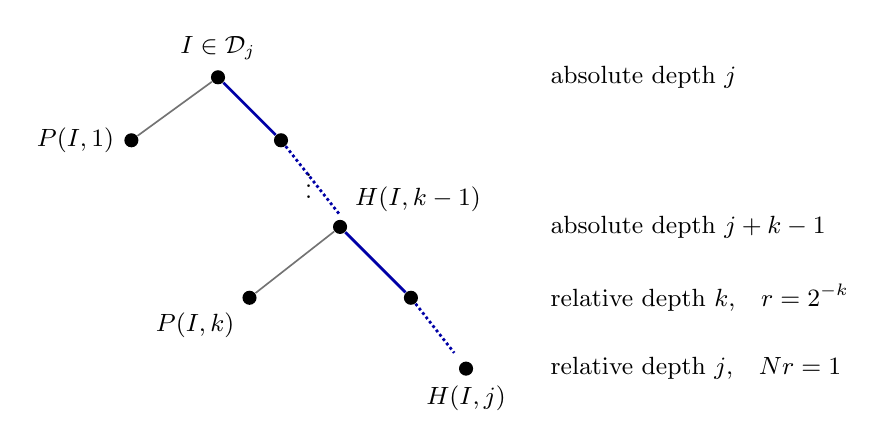
\begin{tikzpicture}[x=1cm,y=1cm,
  dot/.style={circle,fill=black,inner sep=1.8pt},
  heavy/.style={line width=1pt,blue!65!black},
  light/.style={line width=.6pt,black!55},
  every node/.style={font=\small}]
 \node[dot,label=above:{$I\in\mathcal D_j$}] (i) at (0,0) {};
 \node[dot] (h1) at (.8,-.8) {};
 \node[dot,label=left:{$P(I,1)$}] (l1) at (-1.1,-.8) {};
 \draw[heavy] (i)--(h1); \draw[light] (i)--(l1);
 \node at (1.15,-1.28) {$\vdots$};
 \draw[heavy,densely dotted] (h1)--(1.55,-1.75);
 \node[dot,label=above right:{$H(I,k-1)$}] (hk) at (1.55,-1.9) {};
 \node[dot,label=below left:{$P(I,k)$}] (lk) at (.4,-2.8) {};
 \node[dot] (hnext) at (2.45,-2.8) {};
 \draw[light] (hk)--(lk); \draw[heavy] (hk)--(hnext);
 \draw[heavy,densely dotted] (hnext)--(3,-3.5);
 \node[dot,label=below:{$H(I,j)$}] (end) at (3.15,-3.7) {};
 \node[anchor=west] at (4.1,0) {absolute depth $j$};
 \node[anchor=west] at (4.1,-1.9) {absolute depth $j+k-1$};
 \node[anchor=west] at (4.1,-2.8) {relative depth $k$,\quad $r=2^{-k}$};
 \node[anchor=west] at (4.1,-3.7) {relative depth $j$,\quad $Nr=1$};
\end{tikzpicture}

 \caption{A heavier-child path starting at absolute depth $j$.  Its
 lighter child at relative depth $k$ has a parent at absolute depth
 $j+k-1$.  Holding $k$ fixed and changing the frequency index $j$
 therefore selects distinct parent vertices in one common tree.
 The path stops at $k=j$, where the rescaled frequency is $Nr=1$.}
 \label{e:time-tree-figure}
\end{figure}

\Needspace{12\baselineskip}
\begin{theorem}[Local $L^1$ endpoint maximal estimate]
\label{e:maximal}
For compactly supported $\widehat f\in L^2$ and every unit ball $\Omega$,
\begin{equation}
 \int_\Omega\sup_{0\le t<1}|S(t)f(x)|\dd x
       \le C\norm{f}_{H^s(\R^n)}.
 \label{e:maximal-formula}
\end{equation}
The constant is uniform under translation of $\Omega$.
\end{theorem}

\begin{proof}
Take a smooth inhomogeneous Littlewood--Paley decomposition
$f=f_{\mathrm{lo}}+\sum_{j\ge1}f_{2^j}$ with bounded frequency overlap.
The low-frequency part satisfies
$\sup_{x,t}|S(t)f_{\mathrm{lo}}(x)|\le C\norm{f_{\mathrm{lo}}}_2$.
For a fixed measurable graph $t(x)$ and phase $w(x)$, frequency
Cauchy--Schwarz and \Cref{e:dual-square} give
\begin{align*}
 \left|\int_\Omega w(x)\sum_jS(t(x))f_{2^j}(x)\dd x\right|
 &\le C\left(\sum_j2^{2js}\norm{f_{2^j}}_2^2\right)^{1/2}
        \left(\sum_j2^{-2js}\norm{G_{2^j}([0,1))}_2^2\right)^{1/2}\\
 &\le C\norm{f}_{H^s}.
\end{align*}
Choose the annular cutoff in $G_{2^j}$ equal to one on the corresponding
Littlewood--Paley support.  The first factor is the Sobolev square sum;
no frequency logarithm or $\ell^1$ sum has appeared.
For a finite time list, select the first maximizer of the full field
and its conjugate phase (zero where the field is zero).  These are
measurable and are common to every frequency.  The preceding bound is
then the integral of that finite maximum.  Increase the lists to a
dense countable subset of $[0,1)$ containing zero.  Continuity of the
bounded-frequency field and monotone convergence prove
\eqref{e:maximal-formula}.  All kernel estimates depend only on spatial
differences, giving the asserted translation uniformity.
\end{proof}

\subsection{One representative and all real times}
\label{e:trace}

To complete \Cref{m:main}, we first construct a representative continuous
in time and then remove Gaussian regularization uniformly in time on
one full-measure spatial set.  The following approximate-identity lemma
will be applied to a countable family of error envelopes.

\begin{lemma}[Gaussian approximation with uniform local integrals]
\label{e:gaussian-local}
Let $M\ge0$ be measurable and
$A=\sup_z\int_{B(z,1)}M<\infty$.  For
\[
 K_a(y)=(4\pi a)^{-n/2}e^{-|y|^2/(4a)},\qquad a>0,
\]
the convolution $K_a*M$ is finite at every point.  At every Lebesgue
point $x$ of $M$, it tends to $M(x)$ as $a\downarrow0$.
\end{lemma}

\begin{proof}
For a fixed $\rho>0$, cover each annulus
$2^\ell\rho\le|y|<2^{\ell+1}\rho$ by
$C(1+2^\ell\rho)^n$ unit balls.  Uniformly in the center $x$,
\begin{equation}
 \int_{|y|\ge\rho}K_a(y)M(x-y)\dd y
 \le C A a^{-n/2}\sum_{\ell\ge0}(1+2^\ell\rho)^n
                    e^{-4^\ell\rho^2/(4a)}.
 \label{e:gaussian-annuli}
\end{equation}
The series is finite for every $a>0$, and for all sufficiently small
$a$ it is at most $C_\rho A a^{-n/2}e^{-\rho^2/(8a)}$.
The integral over a bounded ball is finite by local integrability,
which proves the first assertion.

At a Lebesgue point set
$H_x(r)=\int_{|y|<r}|M(x-y)-M(x)|\dd y=o(r^n)$.
Given $\eps>0$, choose $\rho$ so that $H_x(r)\le\eps r^n$ for
$0<r\le\rho$.  Radial integration by parts gives
\[
 \int_{|y|<\rho}K_a(y)|M(x-y)-M(x)|\dd y
 \le \eps\left(K_a(\rho)\rho^n+
                  \int_0^\rho(-K_a'(r))r^n\dd r\right)
 \le C\eps.
\]
The complementary integral tends to zero by
\eqref{e:gaussian-annuli}, together with the elementary Gaussian tail
bound for the constant $|M(x)|$.  Letting $\eps\downarrow0$ proves the
claim.
\end{proof}

\Needspace{8\baselineskip}
\begin{proof}[Proof of \Cref{m:main}]
Fix $n\ge3$ and a complex-valued $f\in H^s(\R^n)$.
Choose $f_j$ with $\widehat f_j\in C_c^\infty$ and
$\norm{f_j-f}_{H^s}\le2^{-j}$.  The successive differences satisfy a
summable $H^s$ bound.  By \Cref{e:maximal}, on every unit ball
\[
 \int\sum_j\sup_{0\le t<1}|S(t)(f_{j+1}-f_j)(x)|\dd x<\infty.
\]
A countable covering of $\R^n$ therefore gives a common full-measure
set $E_0$ on which $S(t)f_j(x)$ converges uniformly for $0\le t<1$.
Call the limit $v(x,t)$ and set $v(x,t)=0$ off $E_0$.  For every $x$,
$v(x,\cdot)$ is continuous on $[0,1)$; it is jointly measurable as a
pointwise limit on a measurable set.  The measurability of $E_0$ and of
all the suprema just used can equally be read from the countable dense
set of times, by continuity.

Fix an arbitrary real $t\in[0,1)$.  Unitarity gives
$S(t)f_j\to S(t)f$ in $L^2$, whereas the construction gives pointwise
convergence to $v(\cdot,t)$ almost everywhere.  Hence $v(\cdot,t)$ is
an $L^2$ representative of $S(t)f$.  For each $a>0$ and $x\in\R^n$,
the function $K_a(x-\cdot)$ lies in $L^2$.  Pairing it with this
$L^2$ class and using Plancherel yields the everywhere-defined identity
\begin{equation}
 U_a f(x,t)=(K_a*v(\cdot,t))(x).
 \label{e:class-gaussian-identity}
\end{equation}
The fixed $t$ was arbitrary.  Thus \eqref{e:class-gaussian-identity}
holds for every triple $(x,a,t)$ in the indicated ranges; no
intersection of time-dependent exceptional sets has been taken.
The convolution is absolutely convergent by Cauchy--Schwarz.

Let
\[
 M_j(x)=\sup_{0\le t<1}|v(x,t)-S(t)f_j(x)|.
\]
These functions are measurable because the supremum equals the one
over rational times.  They tend to zero on $E_0$.  Uniform convergence
there and Fatou's lemma applied to
$\sup_t|S(t)(f_\ell-f_j)|$ show that
\begin{equation}
 A_j:=\sup_z\int_{B(z,1)}M_j(x)\dd x
       \le C\norm{f-f_j}_{H^s}.
 \label{e:envelope-local-integrals}
\end{equation}
All translated balls have the same constant by \Cref{e:maximal}.
The values on the null complement of $E_0$ do not affect this estimate.
Intersect $E_0$ with the Lebesgue-point sets of the countably many
$M_j$.  By \Cref{e:gaussian-local}, at every point of this intersection
$K_a*M_j(x)\to M_j(x)$ for every $j$.

For every $y$ and every $t$, the definition of $M_j$ gives the
simultaneous inequality $|v(y,t)-S(t)f_j(y)|\le M_j(y)$.
Combining it with \eqref{e:class-gaussian-identity} gives
\begin{equation}
 \sup_{0<t<1}|U_a f(x,t)-v(x,t)|
 \le (K_a*M_j)(x)+M_j(x)+R_j(a),
 \label{e:envelope-gaussian-bound}
\end{equation}
where
\[
 R_j(a):=(2\pi)^{-n}
     \int |1-e^{-a|\xi|^2}|\,|\widehat f_j(\xi)|\dd\xi
       \longrightarrow0.
\]
This last convergence is uniform in $x,t$ since
$\widehat f_j\in L^1$.  First let $a\downarrow0$ at a point of the
common set.  The limsup of the left side of
\eqref{e:envelope-gaussian-bound} is at most $2M_j(x)$.
Then let $j\to\infty$.  This proves
\eqref{m:eq-uniform-Gaussian} for all real times in the interval
at once.

Finally, intersect with the Lebesgue points of $f$ and with the
full-measure set on which $v(x,0)=f(x)$, supplied by the fixed-time
$L^2$ identity at zero.  On the resulting $E_f$,
$v(x,0)=f^*(x)$ and time continuity gives
$v(x,t)\to f^*(x)$ as real $t\downarrow0$.
The Gaussian limit in \eqref{m:eq-uniform-Gaussian} is taken first,
so these are exactly the asserted iterated limits.
\end{proof}
